\documentclass[10pt,UKenglish, leqno, xcolor = dvipsnames]{beamer}

\usetheme{UiB}

% Font choice:
\usefonttheme{default}

\usepackage{cite}
\usepackage{subfig}
\usepackage{amsmath, amsthm, mathtools, color, setspace}
\usepackage{fancyhdr, braket, etoolbox,booktabs,multirow}
\usepackage{xfrac, lmodern, ifsym, bm, multicol, booktabs, pdflscape}
\usepackage[utf8]{inputenx} % For æ, ø, å
\usepackage{csquotes}       % Quotation marks
\usepackage{microtype}      % Improved typography
\usepackage{amssymb}        % Mathematical symbols
\usepackage{mathtools,physics,centernot,tensor}      % Mathematical symbols
\usepackage[absolute, overlay]{textpos} % Arbitrary placement
\setlength{\TPHorizModule}{\paperwidth} % Textpos units
\setlength{\TPVertModule}{\paperheight} % Textpos units
\usepackage[dvipsnames]{xcolor}
\usepackage{tikz}
\usetikzlibrary{tikzmark,calc,overlay-beamer-styles,arrows,shapes}  % Overlay effects for TikZ
\newenvironment{proenv}{\only{\setbeamercolor{local structure}{fg=RoyalBlue}}}{}
\newenvironment{conenv}{\only{\setbeamercolor{local structure}{fg=Maroon}}}{}
\newenvironment{bibbianoenv}{\only{\setbeamercolor{local structure}{fg=Green}}}{}
\DeclarePairedDelimiter{\insieme}{\{}{\}}
\newcommand{\numberset}{\mathbb}
\newcommand{\alg}{\mathfrak}
\newcommand{\Z}{\numberset{Z}}
\newcommand{\R}{\numberset{R}}
\newcommand{\N}{\numberset{N}}
\newcommand{\C}{\numberset{C}}
\newcommand{\A}{\alpha}


\usetikzlibrary{chains, positioning, shapes.symbols}
\tikzset{start/.style = {signal, 
						fill=#1,
						draw=white,
						font=\tiny,
						text=white,
						inner sep=2pt,
						signal pointer angle=90,
		 				on chain},
						cont/.style = {start=#1, signal from=west}
		}

\usepackage{tcolorbox}
\newtcolorbox{box1}[1]{colback=white!5!white,colframe=green!60!white,fonttitle=\bfseries,title=#1}
\newtcolorbox{box2}[1]{colback=white!5!white,colframe=red!60!gray,fonttitle=\bfseries,title=#1}

\author{Pietro Daniele}
\title{\large Search for new resonances in the 100 to 195 GeV diphoton invariant mass range using 140 fb$^{-1}$ of $pp$ collisions collected at $\sqrt{s}$=13 TeV with the ATLAS detector}

\begin{document}
	\tikzstyle{na} = [baseline=-.5ex]
	\tikzstyle{every picture}+=[remember picture]
	
	\begin{frame}{LHC}
		\vfill
		\begin{itemize}
			\item The \textit{Large Hadron Collider} (LHC) \\is a protons and heavy ions collider\\ installed in the 27 km long LEP \\tunnel
			\item Run2 $pp$ collisions $\sqrt{s} = 13$ TeV
			\item Four leading experiments installed\\ in the four $pp$ interaction points:
			\begin{itemize}
				\item \textbf{ATLAS}
				\item CMS
				\item LHCb
				\item ALICE
			\end{itemize}
		\end{itemize}
		\vfill
		\begin{textblock}{1.}(0.5,.2)
			\includegraphics[width=.5\textwidth]{../thesis_images/CERN_complex.png}
		\end{textblock}
	\end{frame}

	\begin{frame}{ATLAS}
		\vfill
		The ATLAS experiment:
		\begin{itemize}
			\item a multi purpose detector
			\item forward-backward symmetric detector with a $\sim4\pi$ angular coverage
			\item composed of several layers:
			\begin{itemize}
				\item Inner Detector (ID)
				\item Calorimetric system
				\item Muon Spectrometer
			\end{itemize}
			\item Magnetic field:
			\begin{itemize}
				\item a solenoid
				\item a barrel toroid and\\ two end-cap toroids
			\end{itemize}
			\item Trigger system
			\begin{itemize}
				\item 40 MHz $\to$ 1 kHz
			\end{itemize}
			
		\end{itemize}
		\vfill
		\begin{textblock}{1.}(0.375,.45)
			\includegraphics[width=.575\textwidth]{../thesis_images/ATLAS.png}
		\end{textblock}
	\end{frame}

	\begin{frame}{Standard Model (SM)}
		\vfill
		The Standard Model of particle physics is a quantum field theory:
		\begin{itemize}
			\item based on SU(2)$_L\otimes$U(1)$_Y\otimes$SU(3)$_C$\\ gauge symmetry
			\item explains the basic building blocks of\\ matter interactions
			\item classifies all the subatomic known\\ particles
			\item predicted new particles:
			\begin{itemize}
				\item gluon
				\item top ($t$) and charm ($c$) quarks
				\item $W$ and $Z$ bosons $\leftarrow$ \textit{massless}
			\end{itemize}
		\end{itemize}
		$W$ and $Z$ bosons discovered in 1983
		$
		\begin{cases}
			m_W = 80\ GeV\\
			m_Z = 91\ GeV\\
		\end{cases}
		$\\
		$\Rightarrow$ the introduction of $W,Z$ mass terms in the SM Lagrangian would break the local gauge invariance of the theory\\ 
		\begin{center}
			$\Rightarrow$ \textit{Spontaneous Symmetry Breaking}\\
			$\Rightarrow$ \textbf{Higgs Boson}
		\end{center}
		\vfill
		\begin{textblock}{1.}(0.525,.175)
			\includegraphics[width=.45\textwidth]{../thesis_images/SM.jpeg}
		\end{textblock}
	\end{frame}

	\begin{frame}{Higgs boson discovery}
		\vfill
		Higgs boson:
		\begin{itemize}
			\item a massive scalar boson
			\item spin-0
			\item no electric and colour charge
			\item couples only to massive particles
			\item discovered by the ATLAS and CMS\\ experiments in July 2012:
			\begin{itemize}
				\item $m_H$ = 125.09$\pm$0.24 GeV (Run1)
				\item the $H \to \gamma\gamma$ channel was used\\ in the ATLAS experiment
				\begin{itemize}
					\item Non resonant background
					\item final state kinematic fully\\ reconstructed
					\item Excellent invariant mass\\ resolution (1-2 GeV)
				\end{itemize}
			\end{itemize}
		\end{itemize}
		\vfill
		\begin{textblock}{1.}(0.525,.125)
			\includegraphics[width=.45\textwidth]{../thesis_images/higgs_boson_plot.png}
		\end{textblock}
		\begin{textblock}{1.}(0.6,.63)
			\begin{itemize}
				\footnotesize
				\item Irr $\to$ QCD di-photon production
				\vspace{.2cm}
				\item Red $\to$ ($\gamma$,jet), (jet,jet) with jet\\ misidentification (\textit{fake rate})
			\end{itemize}
		\end{textblock}
		\begin{textblock}{1.}(.45,.6125)
			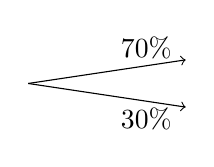
\begin{tikzpicture}
				\draw[-to] (0,0) -- (2.,0.3);
				\path (1.5,0.45) node {70\%};
				\draw[-to] (0,0) -- (2.,-0.3);
				\path (1.5,-0.45) node {30\%};
			\end{tikzpicture}
		\end{textblock}
	\end{frame}

	\begin{frame}{SM limitations}
		\vfill
		SM is not the final theory of nature:
		\begin{itemize}
			\item no dark matter candidate  
			\item no explanation for the matter-antimatter\\ asymmetry 
		\end{itemize}
		\begin{textblock}{1.}(.6,.26)
			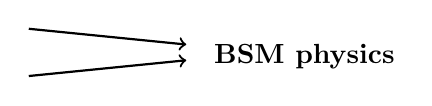
\begin{tikzpicture}
				\draw[-to,thick] (0,.8) -- (2,0.6);
				\draw[-to,thick] (0,.2) -- (2,0.4);
				\path (3.5,0.45) node {\textbf{BSM physics}};
			\end{tikzpicture}
		\end{textblock}
		\vspace{1cm}
		Higgs field:
		\begin{itemize}
			\item a complex doublet under SU(2)$_L$ symmetry group
			\item could be extended $\Rightarrow$ larger scalar sectors:
			\begin{itemize}
				\item BSM resolution
				\item Higgs sector
				\item additional structures $\Rightarrow$ \textbf{NEW BOSONS}
				\item new theory
				\begin{itemize}
					\item 2HDM $\leftarrow$ \textit{bottom-up} approach
					\item SUSY $\leftarrow$ \textit{top-down} approach
				\end{itemize}
			\end{itemize} 
		\end{itemize}
		\vfill
	\end{frame}
		
	\begin{frame}{New spin-0 resonances analysis}
		\vfill
		\begin{center}
			BSM physics $\Rightarrow$ New spin-0 resonances search
		\end{center}
		\begin{itemize}
			\item \textbf{Channel}: $H \to \gamma\gamma$
			\item \textbf{Aim}: find an excess of events over\\ the expected background
			\item \textbf{Signal}:
			\begin{itemize}
				\item $X \to \gamma\gamma$ 
				\item a function of the resonance\\ mass $m_X$
				\item small SM assumptions
			\end{itemize}
			\item \textbf{Background}
			\begin{itemize}
				\item Non resonant background
				\item SM Higgs boson background
			\end{itemize}
		\end{itemize}
		\vfill 
		\begin{textblock}{1}(.45,.4)
			\includegraphics[width=.6\textwidth]{../thesis_images/HSM_prova.pdf}
		\end{textblock}
		\begin{textblock}{1}(.575,.46)
			\colorbox{white}{
				\begin{minipage}{3.cm}
					\tiny
					Template $\mu$=1 and $m_X$=140 GeV\\
					Background+signal$_{\mu=1}^{m_X=140 GeV}$\\
					$m_{\gamma\gamma} \epsilon$ [100,195] GeV\\
					\textit{Inclusive}
				\end{minipage}
			}
		\end{textblock}
		
		\begin{textblock}{1.}(.2,.425)
			\begin{tikzpicture}
				\draw[-to,purple] (0,2.75) -- (6.5,0);
			\end{tikzpicture}
		\end{textblock}
		\begin{textblock}{1.}(.425,.6)
			\begin{tikzpicture}
				\draw[-to,yellow] (0,-.75) -- (1.5,0);
			\end{tikzpicture}
		\end{textblock}
		\begin{textblock}{1.}(.45,.7)
			\begin{tikzpicture}
				\draw[-to,blue] (0,-2) -- (2.3,0);
			\end{tikzpicture}
		\end{textblock}
	\end{frame}
	
	\begin{frame}{Signal model SM independence}
		\vfill
		New physics search:\\
		$\Rightarrow$  An analysis as much independent as possible from assumptions based on Standard Model
		\begin{itemize}
			\item the SM Higgs production modes are: \textit{ggF}, \textit{VBF}, \textit{WH}, \textit{ZH}...
			\item only \textit{ggF} is considered for the signal model creation
			\item other production modes included as a signal yield systematic uncertainty $\sigma^{prod\ modes}$
		\end{itemize}
		\vspace{1cm}
		\resizebox{.5\textwidth}{1.3cm}{
			\begin{box1}{Advantages}
				\begin{itemize}
					\item small assumptions on the production modes for the new resonances
					\item include and parameterise the ignorance of the relative importance of different production modes for additional scalar Higgs bosons searches.
				\end{itemize}
			\end{box1}
		}\resizebox{.5\textwidth}{1.3cm}{
			\begin{box2}{Disadvantages}
				\begin{itemize}
					\item $\sigma^{prod\ modes}$ increases in the more granular categorisation\\
					$\Rightarrow$ the analysis performances decrease
					\item No Higgs discovery Run1 categorisation
				\end{itemize}
			\end{box2}
		}
		\vfill
		\begin{textblock}{1}(0.,.85)
			\begin{figure}
				\resizebox{\textwidth}{!}{
					\begin{tikzpicture}[
						node distance = 0mm,
						start chain = going right,
						]
						\node[start=gray!20!white, scale=1] {Categories};
						\node[cont=uibblue!80!black,   scale=1] {Sig model};
						\node[cont=gray!20!white,   scale=1] {Bkg model};
						\node[cont=gray!20!white,   scale=1.1] {HSM model};
						\node[cont=gray!20!white,   scale=1] {Syst uncs};
						\node[cont=gray!20!white,   scale=1] {Exp results};
					\end{tikzpicture}		
				}
			\end{figure}
		\end{textblock}
	\end{frame}
	
	\begin{frame}{Events Selection}
		\vfill
		$H \to \gamma\gamma$ channel: \textbf{Event selected}
		\begin{itemize}
			\item $m_{\gamma\gamma}\ \epsilon\ [100,195]$ GeV
			\item two photons:
			\begin{itemize}
				\item identified
				\item isolation
				\item $p_T^{\gamma_i}/m_{\gamma\gamma}$
				%\item $p_T^{\gamma_1}/m_{\gamma\gamma}$ > 0.3 
				%\item $p_T^{\gamma_2}/m_{\gamma\gamma}$ > 0.25
			\end{itemize}
		\end{itemize}
		\begin{textblock}{1}(.2,.2)
			\begin{table}[tbp]
				\centering
				\resizebox{7cm}{!}{
					\small
					\begin{tabular}{llcc}
						\toprule[1.5pt]
						Parameter									& Name						& Reconstruction Level	& Truth Level		\\
						\midrule
						$|\eta^{\gamma_i}|$							& $\eta$ cut				& $<2.37$ 				& $<2.37$			\\
						$p_T^{\gamma_1}/m_{\gamma\gamma}$			& Scalar relative $p_T$ cut & > 0.3					& > 0.3    			\\
						$p_T^{\gamma_2}/m_{\gamma\gamma}$			& Scalar relative $p_T$ cut & > 0.25				& > 0.25			\\
						$E_{T}^{cone20\ \gamma_i}/p_T^{\gamma_i}$ 	& Isolation cut 			& < 0.065				& < 0.065 			\\
						$p_{T}^{cone20\ \gamma_i}/p_T^{\gamma_i}$ 	& Isolation cut 			& < 0.05				& 		 			\\
						\bottomrule[1.5pt]
					\end{tabular}
				}
			\end{table}
		\end{textblock}
		\vspace{.5cm}
		\centering
		$\Downarrow$
		\begin{enumerate}\centering
			\item Categorisation
			\item Signal model
			\item Non-resonant background model
			\item SM Higgs boson background model
			\item Systematic uncertainties
			\item Expected results
		\end{enumerate}
		\vfill
	\end{frame}
	
	\begin{frame}{Categorisation}
		\vfill
		\begin{itemize}
			\item The events are classified into\\ mutually exclusive categories
			\item Designed to enhance the analysis\\ sensitivity
			\begin{itemize}
				\item maximise the signal and\\ bkg ratio $\frac{S}{B}$
				\item minimise the systematic\\ uncertainties
			\end{itemize}
			\item three categorisation test and\\ compared:
			\begin{itemize}
				\item \texttt{Inclusive}, \texttt{catConvEta}, \texttt{catConv}
				\item $\gamma$ conversion status 
				\item $\eta$ position cuts
				\begin{itemize}
					\item central region $|\eta|<0.75$
					\item trans region $ \eta \epsilon [1.3,1.75]$
					\item no central and trans regions
				\end{itemize}
			\end{itemize}
		\end{itemize}
		\begin{textblock}{1}(.5,.15)
			\includegraphics[width=.5\textwidth]{../thesis_images/inclusive_tree.pdf}\\
			\includegraphics[width=.5\textwidth]{../thesis_images/catConvEta_tree.pdf}\\
			\includegraphics[width=.5\textwidth]{../thesis_images/catConv_tree.pdf}\\	
		\end{textblock}	
		\vfill
		\begin{textblock}{1.}(.2,.2125)
			\begin{tikzpicture}
				\draw[-to,black!30] (0,-4) -- (4,0);
			\end{tikzpicture}
		\end{textblock}
		\begin{textblock}{1.}(.35,.425)
			\begin{tikzpicture}
				\draw[-to,black!30] (0,-2) -- (2,0);
			\end{tikzpicture}
		\end{textblock}
		\begin{textblock}{1.}(.45,.67)
			\begin{tikzpicture}
				\draw[-to,black!30] (0,0) -- (0,-0.1)
				node[below] {} -- (.5,-.1);
			\end{tikzpicture}
		\end{textblock}
		\begin{textblock}{1}(0.,.85)
			\begin{figure}
				\resizebox{\textwidth}{!}{
					\begin{tikzpicture}[
						node distance = 0mm,
						start chain = going right,
						]
						\node[start=uibblue!80!black, scale=1] {Categories};
						\node[cont=gray!20!white,   scale=1] {Sig model};
						\node[cont=gray!20!white,   scale=1] {Bkg model};
						\node[cont=gray!20!white,   scale=1.1] {HSM model};
						\node[cont=gray!20!white,   scale=1] {Syst uncs};
						\node[cont=gray!20!white,   scale=1] {Exp results};
					\end{tikzpicture}		
				}
			\end{figure}
		\end{textblock}
	\end{frame}

	\begin{frame}{Signal model}
		\vfill
		For each category:
		\begin{itemize}
			\item \textbf{Function form}: \textit{Double-Sided Crystal\\ Ball} (DSCB):
			\begin{itemize}
				\item a gaussian core + power-law tails
				\item 6 parameters ($\mu, \sigma, a_{1,2}, p_{1,2}$)
			\end{itemize}
			\item \textbf{Samples}: \textit{ggF} MC samples with four\\ different resonance mass $m_X$ (110, 125,\\ 130 and 140 GeV)
			\item \textbf{Fit}: a simultaneous DSCB fit:
			\begin{itemize}
				\item $[100,195]$ GeV $m_{\gamma\gamma}$ range
				\item DSCB parameters $\propto$ $m_X$:\\
				$par(m_X) = A^{par} + B^{par}\cdot m_X$
				\item $A$ and $B$ params fixed after fit\\
			\end{itemize}
		\end{itemize}
		\vspace{.5cm}
		\vfill
		\begin{textblock}{1}(.575,.125)
			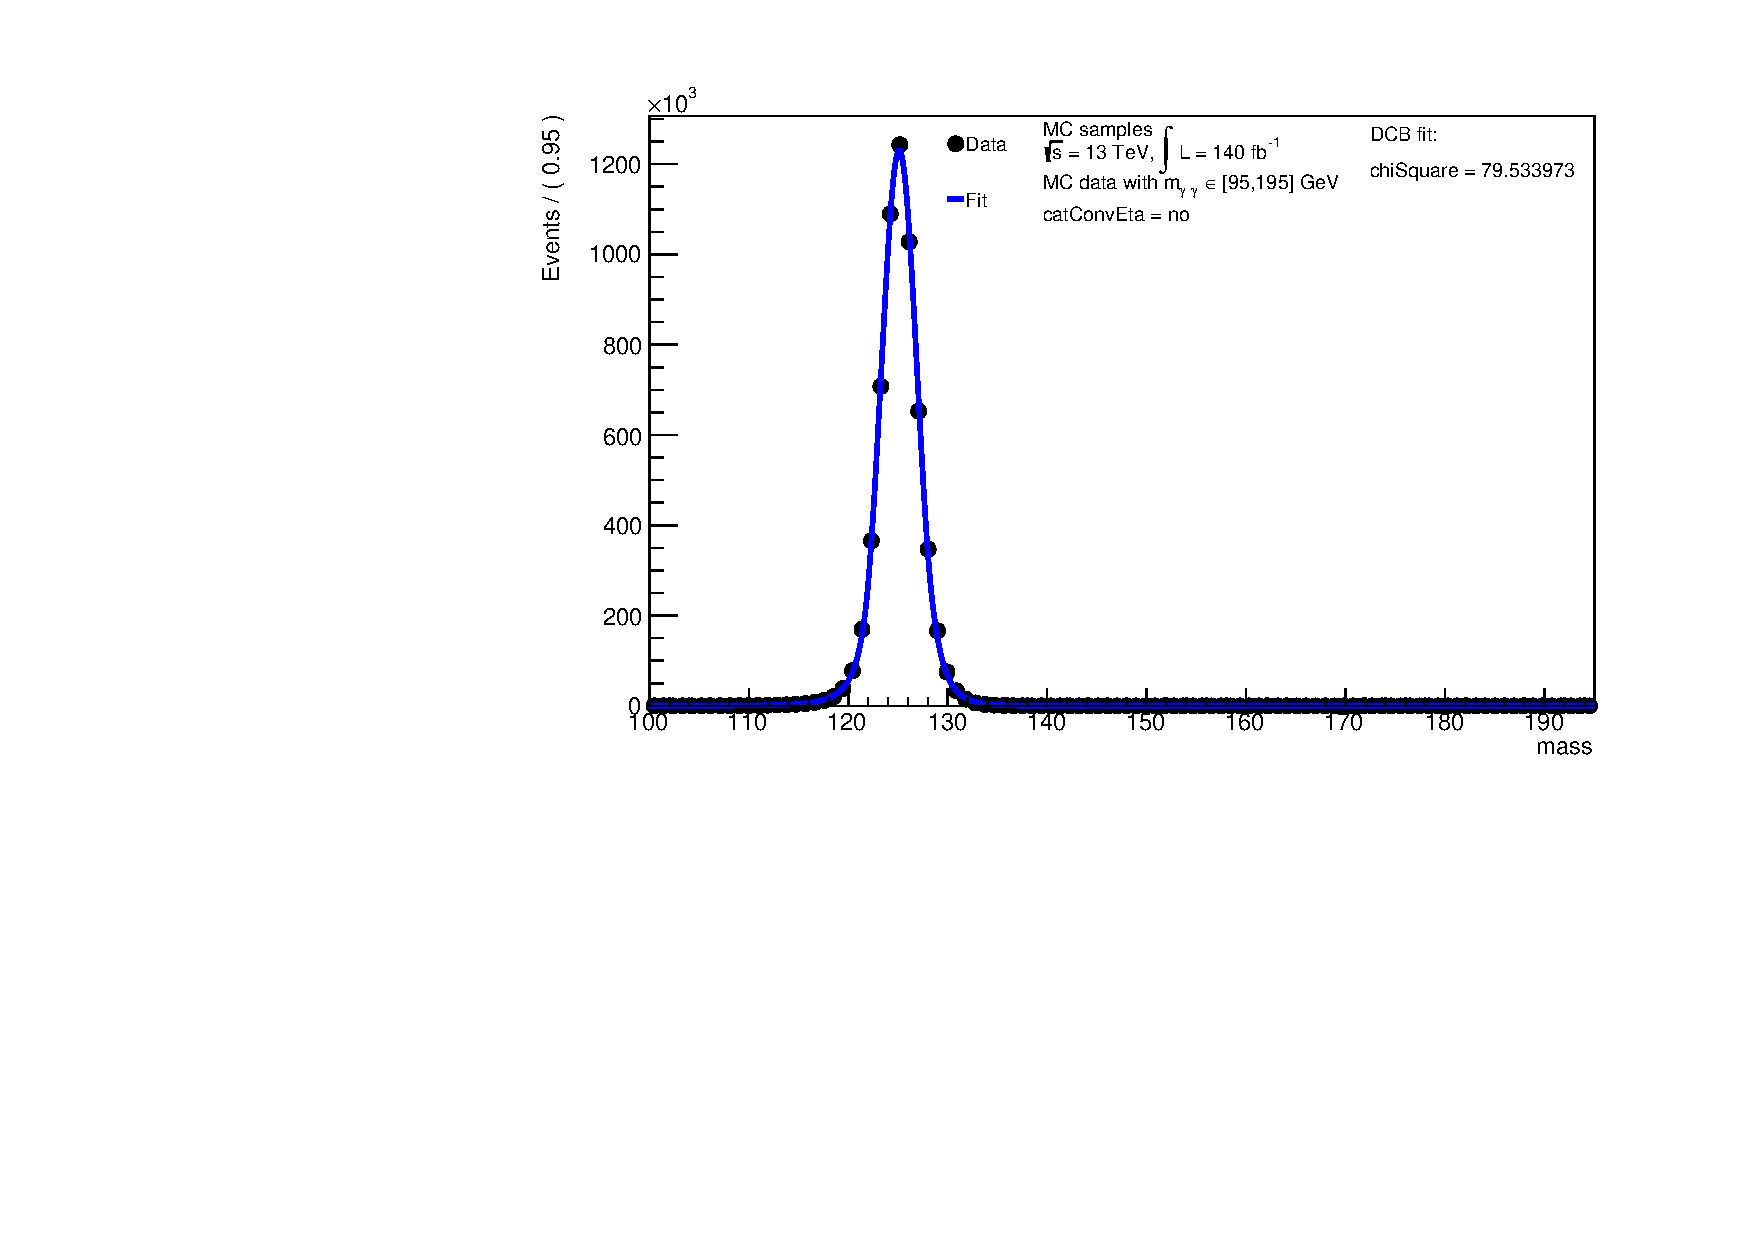
\includegraphics[width=.45\textwidth]{../thesis_images/PowhegPy8_NNLOPS_ggH125_catConvEta_no_fit.pdf}\\
			\includegraphics[width=.45\textwidth]{../thesis_images/sigma_postfit.pdf}\\
		\end{textblock}	
		\begin{textblock}{1}(0.,.85)
			\begin{figure}
				\resizebox{\textwidth}{!}{
					\begin{tikzpicture}[
						node distance = 0mm,
						start chain = going right,
						]
						\node[start=gray!20!white, scale=1] {Categories};
						\node[cont=uibblue!80!black,   scale=1] {Sig model};
						\node[cont=gray!20!white,   scale=1] {Bkg model};
						\node[cont=gray!20!white,   scale=1.1] {HSM model};
						\node[cont=gray!20!white,   scale=1] {Syst uncs};
						\node[cont=gray!20!white,   scale=1] {Exp results};
					\end{tikzpicture}		
				}
			\end{figure}
		\end{textblock}
	\end{frame}

	\begin{frame}{Signal yield($m_X$)}
		\vfill
		In each category $i$, the signal yield is expressed as:
		$$
		N^i(m_X) = \sigma_{ggF}(m_X) \cdot Br_{\gamma\gamma}(m_X) \cdot \mathcal{L}_{Run2} \cdot A_X(m_X)  \cdot C_X^i(m_X)
		$$
		\vspace{.5cm}\\
		\textit{Fiducial} volume:
		\begin{itemize}
			\item the regions of the detector volume sensitive to the distinctive process signatures
			\item \textit{Fiducial} events:
			\begin{itemize}
				\item criteria applied before the reconstruction $\to$ \textit{Truth level}
				\item fiducial criteria mimic the selection criteria
			\end{itemize}		
		\end{itemize}
		\vfill
		\begin{textblock}{1}(0.,.85)
			\begin{figure}
				\resizebox{\textwidth}{!}{
					\begin{tikzpicture}[
						node distance = 0mm,
						start chain = going right,
						]
						\node[start=gray!20!white, scale=1] {Categories};
						\node[cont=uibblue!80!black,   scale=1] {Sig model};
						\node[cont=gray!20!white,   scale=1] {Bkg model};
						\node[cont=gray!20!white,   scale=1.1] {HSM model};
						\node[cont=gray!20!white,   scale=1] {Syst uncs};
						\node[cont=gray!20!white,   scale=1] {Exp results};
					\end{tikzpicture}		
				}
			\end{figure}
		\end{textblock}
	\end{frame}
	
	\begin{frame}{Non-resonant background}
		\vfill
		For each category:
		\begin{itemize}
			\item modelled using MC samples
			\item \textbf{Functional form}:\\ $f^i_{bkg}(m_{\gamma\gamma},N_{bkg}^i,a^i,b^i) = N_{bkg}^i\cdot\exp^{(a^i\cdot m_{\gamma\gamma}+b^i\cdot m_{\gamma\gamma}^2)}$
			\begin{itemize}
				\item $N^{i}_{bkg}$, $a_i$, $bi$ are free parameters
			\end{itemize} 
			\item \textbf{Sample}: di-photon MC samples
			\item \textbf{Fit}: \textit{exp(poly2)} fit:
			\begin{itemize}
				%\item blind search $\to$ [110,170] GeV\\ $m_X$ range
				\item fit $\to$  [100,195] GeV $m_{\gamma\gamma}$ range
			\end{itemize}
			\item the functional form, chosen using\\ MC samples, will applied to data
		\end{itemize}
		\vspace{.5cm}
		\vfill
		\begin{textblock}{1}(.495,.4)
			\includegraphics[width=.55\textwidth]{../thesis_images/bkg_100_195GeV_fit_catConvEta_no_prova.pdf}\\	
		\end{textblock}
		\begin{textblock}{1}(0.,.85)
			\begin{figure}
				\resizebox{\textwidth}{!}{
					\begin{tikzpicture}[
						node distance = 0mm,
						start chain = going right,
						]
						\node[start=gray!20!white, scale=1] {Categories};
						\node[cont=gray!20!white,   scale=1] {Sig model};
						\node[cont=uibblue!80!black,   scale=1] {Bkg model};
						\node[cont=gray!20!white,   scale=1.1] {HSM model};
						\node[cont=gray!20!white,   scale=1] {Syst uncs};
						\node[cont=gray!20!white,   scale=1] {Exp results};
					\end{tikzpicture}		
				}
			\end{figure}
		\end{textblock}
	\end{frame}
	
	\begin{frame}{HSM background}
		\vfill
		For each category:
		\begin{itemize}
			\item \textbf{Function form}: \textit{Double-Sided Crystal\\ Ball} (DSCB):
			\begin{itemize}
				\item a gaussian core + power-law tails
				\item 6 parameters ($\mu, \sigma, a_{1,2}, p_{1,2}$)
			\end{itemize}
			\item \textbf{Samples}: all SM Higgs 125 GeV production modes\\ MC sample
			\item \textbf{Fit}: a single DSCB fit:
			\begin{itemize}
				\item DSCB parameters fixed after the fit
				\item $[100,195]$ GeV $m_{\gamma\gamma}$ range
				\item yield set from SM predictions
			\end{itemize}
		\end{itemize}
		\vspace{.75cm}
		\vfill
		\begin{textblock}{1}(.575,.3)
			\includegraphics[width=.45\textwidth]{../thesis_images/bkg/HSM_fit_catConvEta_no.pdf}\\	
		\end{textblock}
		\begin{textblock}{1}(0.,.85)
			\begin{figure}
				\resizebox{\textwidth}{!}{
					\begin{tikzpicture}[
						node distance = 0mm,
						start chain = going right,
						]
						\node[start=gray!20!white, scale=1] {Categories};
						\node[cont=gray!20!white,   scale=1] {Sig model};
						\node[cont=gray!20!white,   scale=1] {Bkg model};
						\node[cont=uibblue!80!black,   scale=1.1] {HSM model};
						\node[cont=gray!20!white,   scale=1] {Syst uncs};
						\node[cont=gray!20!white,   scale=1] {Exp results};
					\end{tikzpicture}		
				}
			\end{figure}
		\end{textblock}
	\end{frame}

	\begin{frame}{Systematic Uncertainties}
		\vfill
		Systematic uncertainties
		\begin{itemize}
			\item arise from experimental sources
			\item specific for each category
			\item  are included into the likelihood model of the measurement as nuisance parameters
			\item divided into two different groups:
		\end{itemize}
		\vspace{.5cm}
		\begin{enumerate}\centering
			\item shape systematic uncertainties
			\item yield systematic uncertainties
		\end{enumerate}
		\vfill
		\begin{textblock}{1}(0.,.85)
			\begin{figure}
				\resizebox{\textwidth}{!}{
					\begin{tikzpicture}[
						node distance = 0mm,
						start chain = going right,
						]
						\node[start=gray!20!white, scale=1] {Categories};
						\node[cont=gray!20!white,   scale=1] {Sig model};
						\node[cont=gray!20!white,   scale=1] {Bkg model};
						\node[cont=gray!20!white,   scale=1.1] {HSM model};
						\node[cont=uibblue!80!black,   scale=1] {Syst uncs};
						\node[cont=gray!20!white,   scale=1] {Exp results};
					\end{tikzpicture}		
				}
			\end{figure}
		\end{textblock}
	\end{frame}

	\begin{frame}{Shape systematic uncertainties}
		\vfill
		Shape systematic uncertainties $\to$ the\\ modelling of $m_{\gamma\gamma}$ distribution:
		\begin{itemize}
			\item photon energy scale uncertainties:
			\begin{itemize}
				\item affect the peak position ($\mu^{DSCB}$)
				%\item $\delta\mu_c(\pm1\sigma)=\frac{<m_{\gamma\gamma}>_i(\pm1\sigma)}{<m_{\gamma\gamma}>_i}-1$
				\item impact of less than 0.5\%
				%\item only on signal model
			\end{itemize}
			\item photon energy resolution uncertainties
			\begin{itemize}
				\item affect the Gaussian width ($\sigma^{DSCB}$)
				%\item $\delta\sigma_c(\pm1\sigma)=\frac{IQR_i(\pm1\sigma)}{IQR_i}-1$
				\item impact of less than 12\%
				%\item on signal and HSM models
			\end{itemize}
			\item LHC Higgs mass uncertainty
			\begin{itemize}
				\item affect the peak position ($\mu^{DSCB}$)
				\item impact of 0.2\%
				\item only on HSM model
			\end{itemize}
		\end{itemize}
		\vspace{.2cm}
		\vfill
		\begin{textblock}{1}(.575,.125)
			\includegraphics[width=.4\textwidth]{../thesis_images/Syst/var_shape_scale_catConvEta_no.pdf}\\
			\includegraphics[width=.4\textwidth]{../thesis_images/Syst/var_shape_res_catConvEta_no.pdf}\\	
		\end{textblock}	
		\begin{textblock}{1}(0.,.85)
			\begin{figure}
				\resizebox{\textwidth}{!}{
					\begin{tikzpicture}[
						node distance = 0mm,
						start chain = going right,
						]
						\node[start=gray!20!white, scale=1] {Categories};
						\node[cont=gray!20!white,   scale=1] {Sig model};
						\node[cont=gray!20!white,   scale=1] {Bkg model};
						\node[cont=gray!20!white,   scale=1.1] {HSM model};
						\node[cont=uibblue!80!black,   scale=1] {Syst uncs};
						\node[cont=gray!20!white,   scale=1] {Exp results};
					\end{tikzpicture}		
				}
			\end{figure}
		\end{textblock}
	\end{frame}

	\begin{frame}{Yield systematic uncertainties}
		\vspace{.2cm}
		Yield systematic uncertainties $\to$ the expected signal and HSM yields
		\begin{itemize}
			\item the $\gamma$ energy scale and resolution uncertainties on the selection efficiency
			\item the $\gamma$ identification and\\ isolation efficiencies
			\item the efficiency of the\\ diphoton trigger
			\item  the modelling of pile-up\\ in the simulation\\
			\vspace{.1cm}
		\end{itemize}
		$\Rightarrow$ an impact of less than 2\%
		\begin{textblock}{1}(.375,.25)
			\includegraphics[width=.65\textwidth]{../thesis_images/Syst/var_catConvEta_no_sig_fid.pdf}\\	
		\end{textblock}
		\begin{textblock}{1}(0.,.85)
			\begin{figure}
				\resizebox{\textwidth}{!}{
					\begin{tikzpicture}[
						node distance = 0mm,
						start chain = going right,
						]
						\node[start=gray!20!white, scale=1] {Categories};
						\node[cont=gray!20!white,   scale=1] {Sig model};
						\node[cont=gray!20!white,   scale=1] {Bkg model};
						\node[cont=gray!20!white,   scale=1.1] {HSM model};
						\node[cont=uibblue!80!black,   scale=1] {Syst uncs};
						\node[cont=gray!20!white,   scale=1] {Exp results};
					\end{tikzpicture}		
				}
			\end{figure}
		\end{textblock}
	\end{frame}

	\begin{frame}{Yield systematic uncertainties}
		\vspace{.2cm}
		Yield systematic uncertainties $\to$ the expected signal and HSM yields\\
		The production mode dependence $\sigma^{prod\ modes}$
		\begin{itemize}
			\item For each category $C_X^{prod}$ parametrised as functions of $m_X$
			\item $\sigma^{prod\ modes}$
			\begin{itemize}
				\item is maximum of linear\\ fits difference
				\item by varying prod modes\\ and resonance mass
			\end{itemize}
		\end{itemize}
		\begin{textblock}{1}(.4,.35)
			\includegraphics[width=.65\textwidth]{../thesis_images/Signal/cx_all_prod_catConvEta_no.pdf}\\	
		\end{textblock}	
		
		\begin{textblock}{1}(0.,.85)
			\begin{figure}
				\resizebox{\textwidth}{!}{
					\begin{tikzpicture}[
						node distance = 0mm,
						start chain = going right,
						]
						\node[start=gray!20!white, scale=1] {Categories};
						\node[cont=gray!20!white,   scale=1] {Sig model};
						\node[cont=gray!20!white,   scale=1] {Bkg model};
						\node[cont=gray!20!white,   scale=1.1] {HSM model};
						\node[cont=uibblue!80!black,   scale=1] {Syst uncs};
						\node[cont=gray!20!white,   scale=1] {Exp results};
					\end{tikzpicture}		
				}
			\end{figure}
		\end{textblock}
	\end{frame}

	\begin{frame}{Combined maximum likelihood fit}
		After:
		\begin{enumerate}
			\item event selection 
			\item application of the different categorisation
			\item models creation
			\item systematic uncertainties study
		\end{enumerate}
	\end{frame}
	
	\begin{frame}{Expected results}
		\vspace{.4cm}
		$\Longrightarrow$ a combined maximum likelihood fit in all the categories is performed
		\begin{itemize}
			\item investigating the presence of a signal by computing the compatibility of the MC template with\\ the background\\ only hypothesis $p_0$
			%\item assessing limits, in a fiducial region, on the\\ x-s in case no excess of signal is observed.
		\end{itemize}	
		\begin{textblock}{1}(.3,.26)	
			\includegraphics[width=.75\textwidth]{../thesis_images/p0_no_catConvEta.pdf}\\
			%\includegraphics[width=.45\textwidth]{../thesis_images/plot_AsimovData_0_ggHyy_MC_no_catConvEta_syst_HSM_fid_nom_gaus.pdf}	
		\end{textblock}
		\begin{textblock}{1}(0.,.85)
			\begin{figure}
				\resizebox{\textwidth}{!}{
					\begin{tikzpicture}[
						node distance = 0mm,
						start chain = going right,
						]
						\node[start=gray!20!white, scale=1] {Categories};
						\node[cont=gray!20!white,   scale=1] {Sig model};
						\node[cont=gray!20!white,   scale=1] {Bkg model};
						\node[cont=gray!20!white,   scale=1.1] {HSM model};
						\node[cont=gray!20!white,   scale=1] {Syst uncs};
						\node[cont=uibblue!80!black,   scale=1] {Exp results};
					\end{tikzpicture}		
				}
			\end{figure}
		\end{textblock}
	\end{frame}
	
	\begin{frame}{Expected results}
		\vspace{.4cm}
		$\Longrightarrow$ a combined maximum likelihood fit in all the categories is performed
		\begin{itemize}
			%\item investigating the presence of a signal by\\ computing the compatibility of the MC\\ template with the background-only\\ hypothesis $p_0$
			\item assessing limits, in a fiducial region, on the x-s in case no excess of signal is observed.
		\end{itemize}		
		\begin{textblock}{1}(.3,.26)
			%\includegraphics[width=.45\textwidth]{../thesis_images/p0_no_catConvEta.pdf}\\
			\includegraphics[width=.75\textwidth]{../thesis_images/xs_fid_AsimovData_0_ggHyy_MC_catConvEta_syst_HSM_fid_nom_gaus.pdf}	
		\end{textblock}
		\begin{textblock}{1}(0.,.85)
			\begin{figure}
				\resizebox{\textwidth}{!}{
					\begin{tikzpicture}[
						node distance = 0mm,
						start chain = going right,
						]
						\node[start=gray!20!white, scale=1] {Categories};
						\node[cont=gray!20!white,   scale=1] {Sig model};
						\node[cont=gray!20!white,   scale=1] {Bkg model};
						\node[cont=gray!20!white,   scale=1.1] {HSM model};
						\node[cont=gray!20!white,   scale=1] {Syst uncs};
						\node[cont=uibblue!80!black,   scale=1] {Exp results};
					\end{tikzpicture}		
				}
			\end{figure}
		\end{textblock}
	\end{frame}

	\begin{frame}{Expected results}
		\vfill
		\textbf{Without} systematic uncertainties improvement\\ compared to \texttt{Inclusive} category
		\begin{itemize}
			\item discovery potential
			\begin{itemize}
				\item \texttt{catConvEta} $\to$ $\sim$6.3\%
				\item \texttt{catConv} $\to$ $\sim$1.2\%
			\end{itemize}
			\item limits setting
			\begin{itemize}
				\item \texttt{catConvEta} $\to$ $\sim$7.6\%
				\item \texttt{catConv} $\to$ $\sim$2.4\%
			\end{itemize}
		\end{itemize}
		\textbf{With} systematic uncertainties improvement\\ compared to \texttt{Inclusive} category
		\begin{itemize}
			\item limits setting
			\begin{itemize}
				\item \texttt{catConvEta}
				\begin{itemize}
					\item always positive improvement
					\item maximum value 4.2\% at $m_X$=170 GeV
				\end{itemize}
				\item \texttt{catConv}
				\begin{itemize}
					\item not always positive improvement\\
					$\Rightarrow$ should be discarded
				\end{itemize}
			\end{itemize}
		\end{itemize}
		\vspace{.5cm}
		\vfill
		\begin{textblock}{1}(.5825,.1)	
			\includegraphics[width=.45\textwidth]{../thesis_images/p0_exp_imp.pdf}\\
			\includegraphics[width=.45\textwidth]{../thesis_images/imp_nom_gaus.pdf}	
		\end{textblock}
		\begin{textblock}{1}(0.,.85)
			\begin{figure}
				\resizebox{\textwidth}{!}{
					\begin{tikzpicture}[
						node distance = 0mm,
						start chain = going right,
						]
						\node[start=gray!20!white, scale=1] {Categories};
						\node[cont=gray!20!white,   scale=1] {Sig model};
						\node[cont=gray!20!white,   scale=1] {Bkg model};
						\node[cont=gray!20!white,   scale=1.1] {HSM model};
						\node[cont=gray!20!white,   scale=1] {Syst uncs};
						\node[cont=uibblue!80!black,   scale=1] {Exp results};
					\end{tikzpicture}		
				}
			\end{figure}
		\end{textblock}
	\end{frame}

	\begin{frame}{Conclusions}
		\vfill
		\begin{itemize}
			\item The potential of search for new resonances in [100,195] GeV $m_{\gamma\gamma}$ range has been investigated
			\item The best categorisation obtained from the trade-off between performances and SM independence is \texttt{catConvEta}:
			\begin{itemize}
				\item a signal significance ranging from few $\sigma$ to $\sim$12$\sigma$ can be achieved in the search for new spin-0 resonance, assuming the SM mass dependence of the cross-section
				\item the excluded fiducial cross-section for a signal ranges from $\sim$3.4 pb to $\sim$34.6 pb depending on the new resonance mass.
			\end{itemize}
			\item The analysis is still blind so no results based on data have been shown
			\item The results presented in this thesis represent the first step towards the unblinding.
		\end{itemize} 
		\vfill
	\end{frame}

	%%%%%%%%% Backup %%%%%%%%%
	\section{Backup}
	\SectionPage
		
		\begin{frame}{Spontaneous Symmetry Breaking}
			With the \textit{Higgs mechanism} and the \textit{Spontaneous Symmetry Breaking} is possible to introduce a gauge invariant mass term of the $W,Z$ gauge boson
		\end{frame}
	
		\begin{frame}{ATLAS coordinate system}
			
		\end{frame}
	
		\begin{frame}{2HDM and SUSY}
			
		\end{frame}
		
		\begin{frame}{Combined maximum likelihood}
			
		\end{frame}
	
			\begin{frame}{Signal yield($m_X$)}
			\vfill
			In each category $i$, the signal yield is expressed as:
			$$
			N^i(m_X) = \sigma_{ggF}(m_X) \cdot A_X(m_X) \cdot Br_{\gamma\gamma}(m_X) \cdot \mathcal{L}_{Run2} \cdot C_X^i(m_X)
			$$
			\begin{center}
				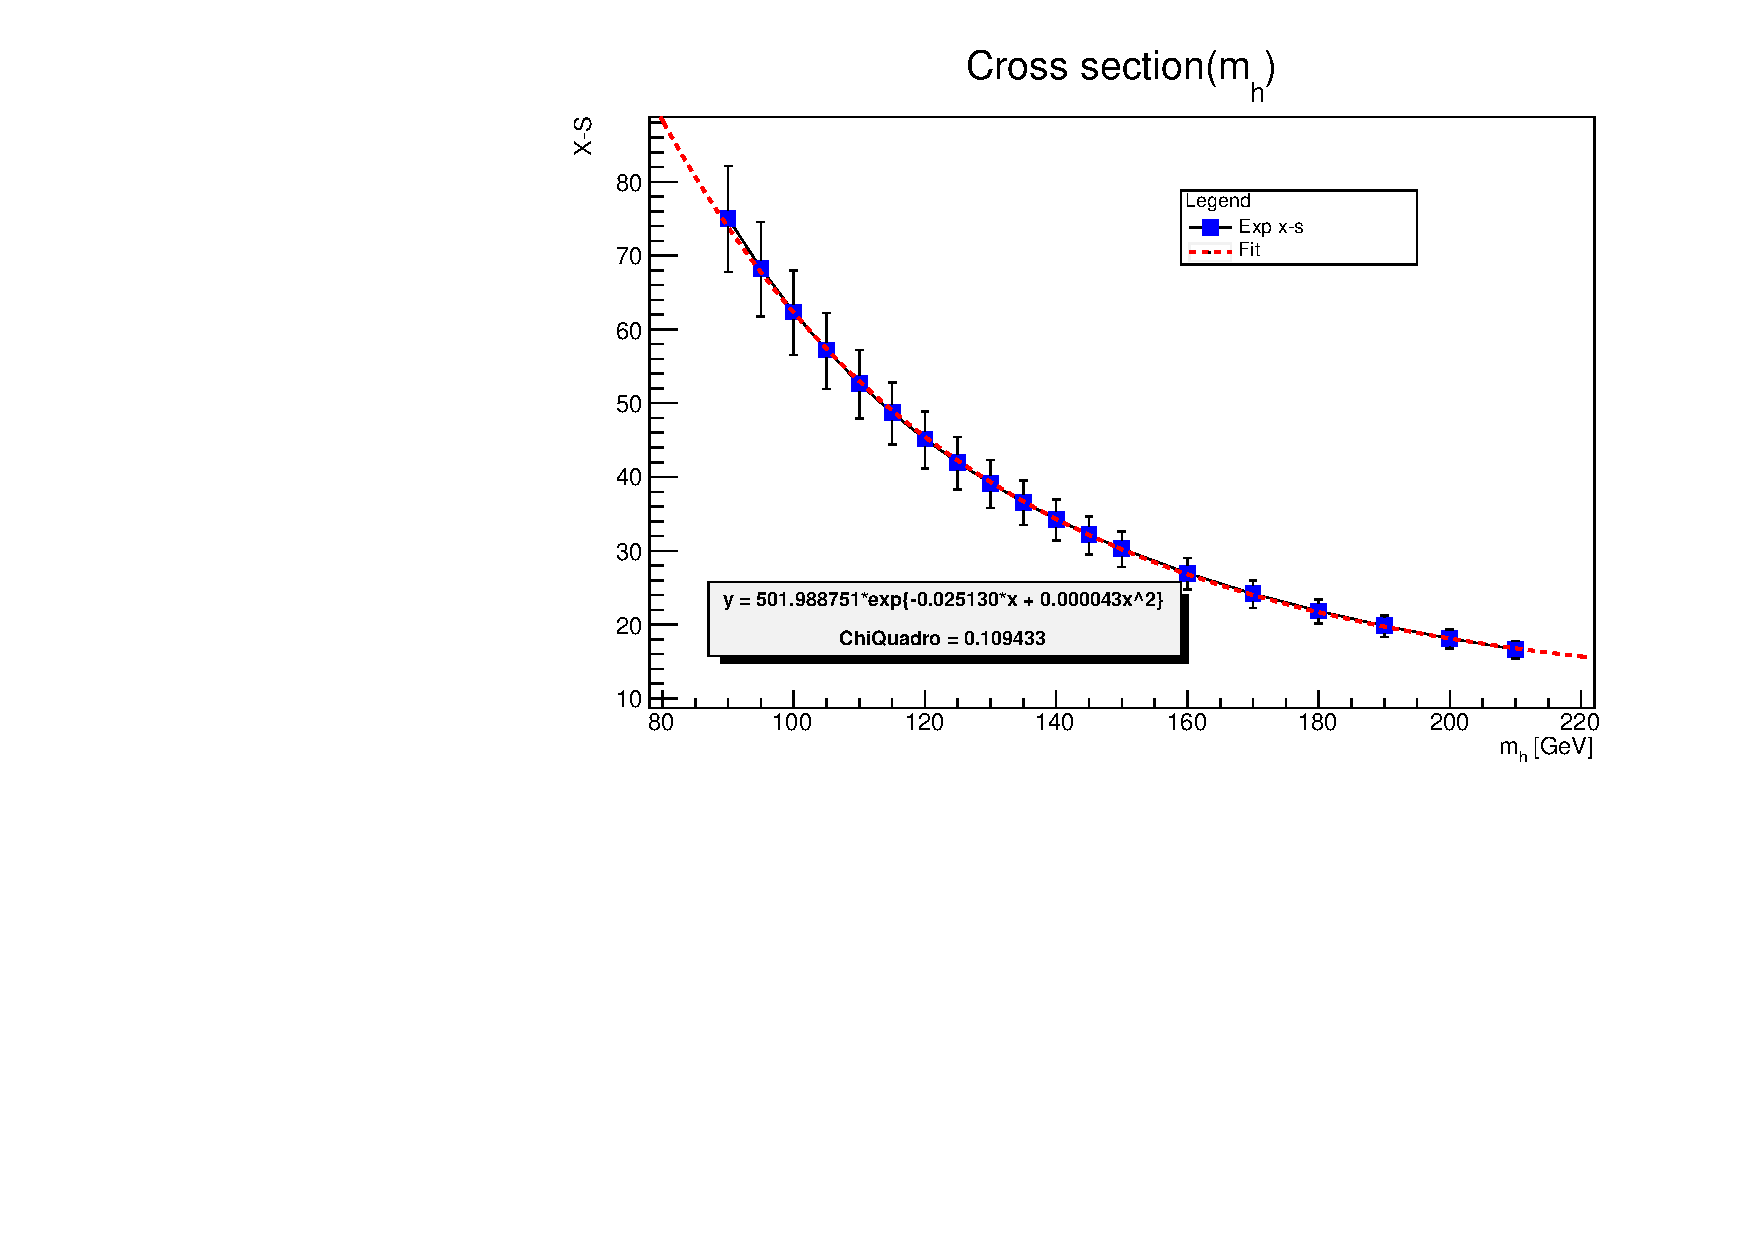
\includegraphics[width=.35\textwidth]{../thesis_images/x_section_fit.pdf}
				\includegraphics[width=.35\textwidth]{../thesis_images/ax_isFiducialMedium_linear_fit.pdf}\\
				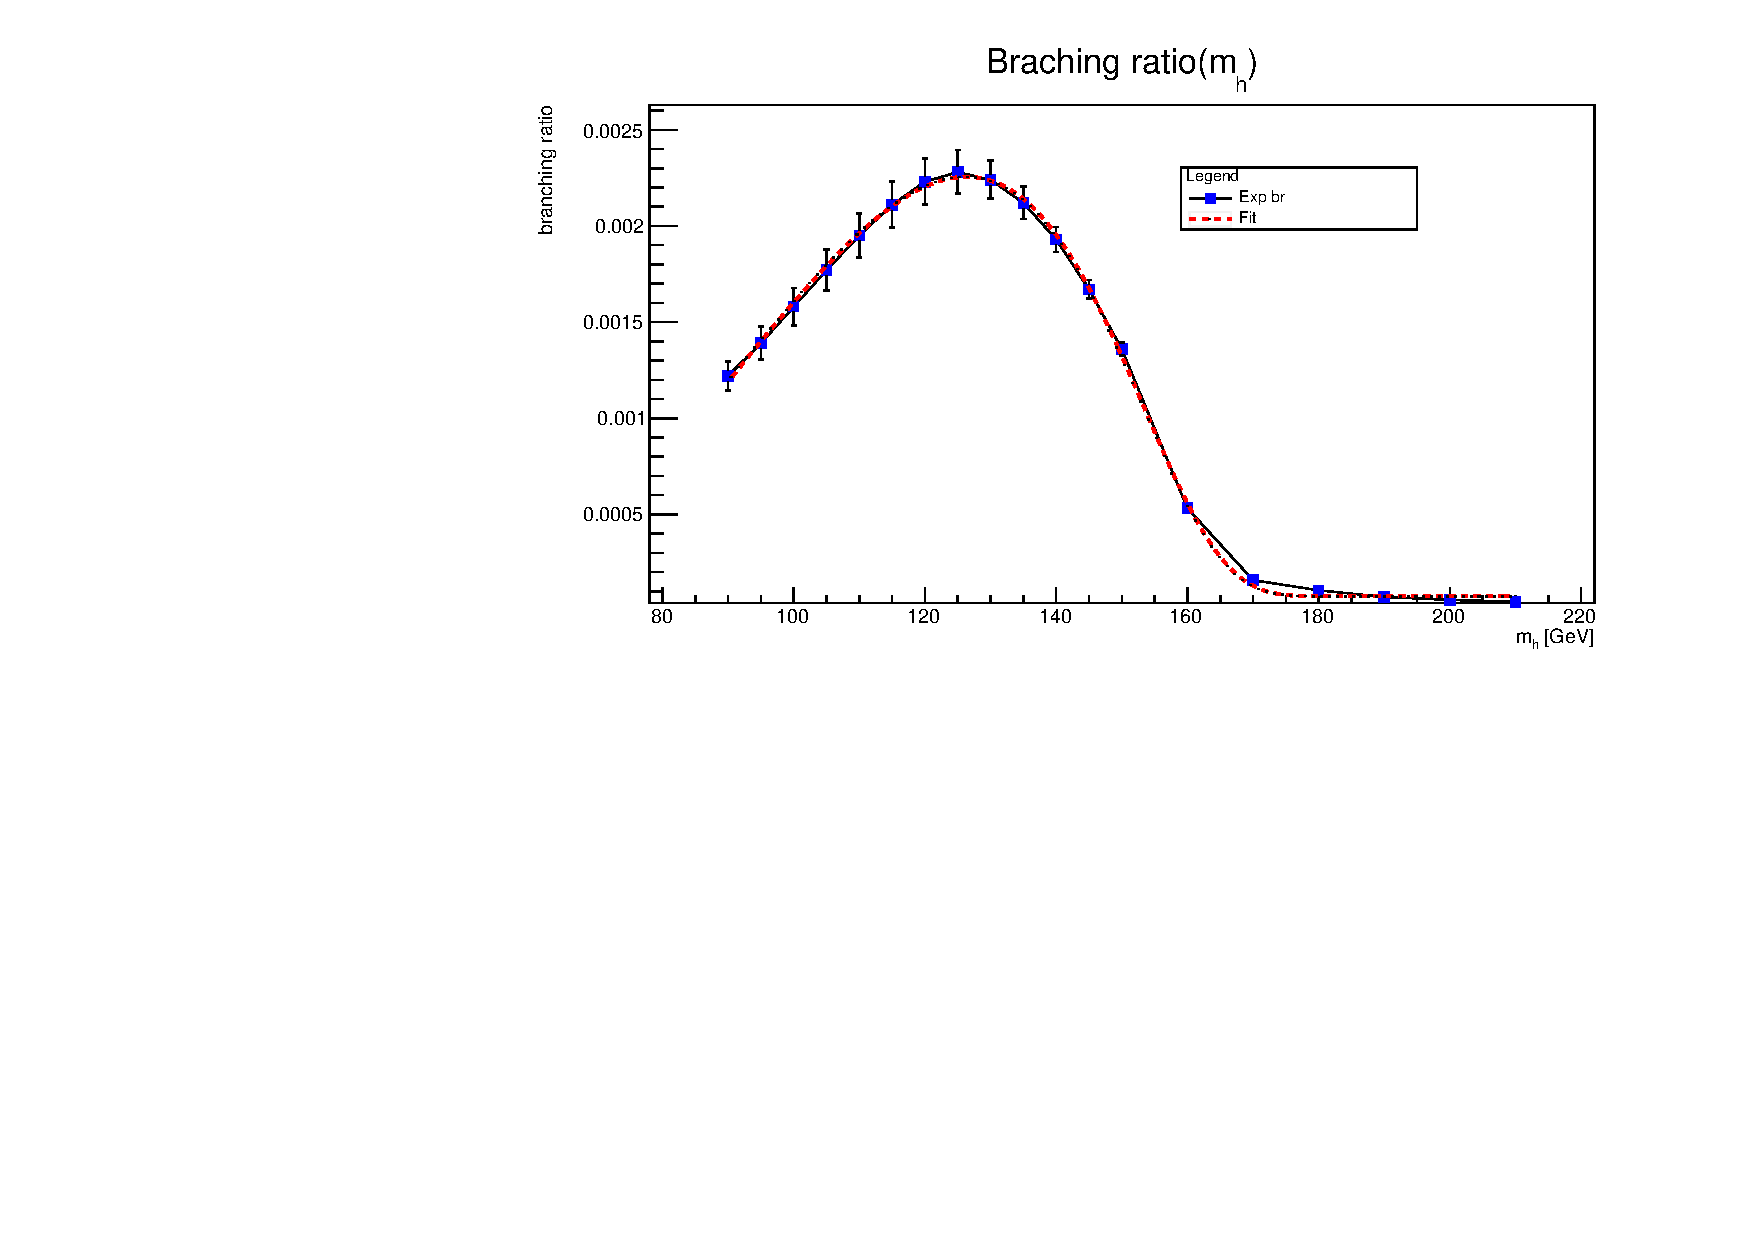
\includegraphics[width=.35\textwidth]{../thesis_images/br_fit.pdf}			
				\includegraphics[width=.35\textwidth]{../thesis_images/cx_fit_catConvEta_no.pdf}
			\end{center}
			\vfill
			\begin{textblock}{1}(0.,.85)
				\begin{figure}
					\resizebox{\textwidth}{!}{
						\begin{tikzpicture}[
							node distance = 0mm,
							start chain = going right,
							]
							\node[start=gray!20!white, scale=1] {Categories};
							\node[cont=uibblue!80!black,   scale=1] {Sig model};
							\node[cont=gray!20!white,   scale=1] {Bkg model};
							\node[cont=gray!20!white,   scale=1.1] {HSM model};
							\node[cont=gray!20!white,   scale=1] {Syst uncs};
							\node[cont=gray!20!white,   scale=1] {Exp results};
						\end{tikzpicture}		
					}
				\end{figure}
			\end{textblock}
		\end{frame}
\end{document}